\section{Preliminary studies}

This section carries out some preliminary studies using Moltres and MOOSE heat conduction module to solve the prismatic HTGR thermal-fluids.

\subsection{Verification of the thermal-fluids model}

To verify our methodology, we apply the equations to a simplified cylindrical model.
Figure \ref{fig:th-ver-mesh} displays the model geometry.
The model differentiates 5 subregions: fuel compact, helium gap, moderator, film, and coolant.
% Material characteristics from ... Need to add citations
We calculated the coolant radius by preserving a coolant channel volume.
We assume a sinusoidal power profile in the $z$-direction.

The analytical solution of this problem is
\begin{align}
  T_c (z) &= T_in + \frac{q_{ave} R_f^2 L}{2 \rho c_p v \pi R_c^2} \left[ 1 + cos \left( \frac{\pi}{L} z \right) \right] \notag \\
  T_3(z) = T_c(z) + \frac{q_{ave} \pi}{2} sin \left( \frac{\pi}{L} z \right) R_f^2 \frac{ln(R_i/R_m)}{2 k_i} \notag \\
  T_2(z) = T_3(z) + \frac{q_{ave} \pi}{2} sin \left( \frac{\pi}{L} z \right) R_f^2 \frac{ln(R_m/R_g)}{2 k_m} \notag \\
  T_1(z) = T_2(z) + \frac{q_{ave} \pi}{2} sin \left( \frac{\pi}{L} z \right) R_f^2 \frac{ln(R_g/R_f)}{2 k_g} \notag \\
  T_f (r=0, z) &= T_1(z) + \frac{q_{ave} \pi}{2} sin \left( \frac{\pi}{L} z \right) R_f^2 \frac{1}{4 k_f} \right] \notag \\
  T_f (r, z=L/2) &= \frac{q_{ave}}{4 k_f} \left(R_f^2 - r^2\right) + T_1 (z=L/2) \notag \\
  T_g (r, z=L/2) &= \frac{T_1 (z=L/2)-T_2 (z=L/2)}{ln (R_f/R_g)} ln (r/R_g) + T_1(z=L/2) \notag \\
  T_m (r, z=L/2) &= \frac{T_2 (z=L/2)-T_3 (z=L/2)}{ln (R_g/R_m)} ln (r/R_m) + T_2(z=L/2) \notag \\
  T_i (r, z=L/2) &= \frac{T_3 (z=L/2)-T_c (z=L/2)}{ln (R_m/R_i)} ln (r/R_i) + T_3(z=L/2) \notag \\
  T_c (r, z=L/2) &= T_c(z=L/2)
  \intertext{where}
  q_{ave} &= \mbox{average power density} = 35 W/cm^3 \notag \\
  R_f &= \mbox{fuel compact radius} = 0.6225 cm \notag \\
  L &= \mbox{fuel column height} = 793 cm \notag \\
  \rho &= \mbox{helium density at 400 $^{\circ}$C and 7 MPa} = 4.94 \times 10^{-6} kg/cm^3 \notag \\
  c_p &= \mbox{helium heat capacity at 400 $^{\circ}$C and 7 MPa} = 5.188 \times 10^{3} J/kg/K \notag \\
  v &= \mbox{average helium velocity} = 1794.33 cm/s \notag \\
  R_c &= \mbox{coolant channel radius} = 0.795 cm \notag \\
  R_g &= \mbox{gap radius} = 0.635 cm \notag \\
  R_m &= \mbox{moderator radius} = 1.08 cm \notag \\
  R_i &= \mbox{film radius} = 1.09 cm \notag \\
  k_f &= \mbox{fuel compact thermal conductivity} = 0.07 W/cm/K \notag \\
  k_g &= \mbox{gap thermal conductivity} = 3 \times 10^{-3} W/cm/K \notag \\
  k_m &= \mbox{moderator thermal conductivity} = 0.3 W/cm/K \notag \\
  k_i &= \mbox{film thermal conductivity} = h R_i ln(R_i/R_m) = 0.001722 W/cm/K \notag \\
\end{align}

Numerical solution of equations shown in Section \ref{ch3:th}.

Figure \ref{fig:th-ver-results} shows the axial and radial temperature profiles.

\begin{figure}[htbp!]
	\centering
	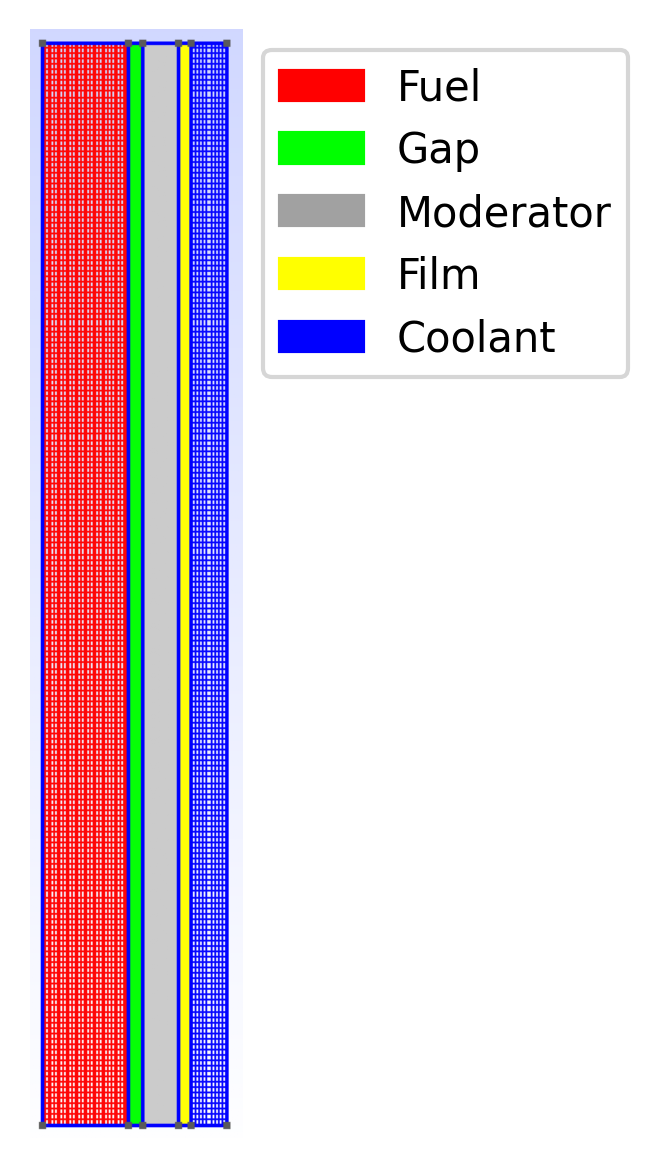
\includegraphics[width=0.35\linewidth]{figures-thermal/2D-preliminar-mesh2}
	\hfill
	\caption{Scaled-down version of the geometry.}
	\label{fig:th-ver-mesh}
\end{figure}

\begin{figure}[htbp!]
	\centering
    \subfloat[Fuel centerline and coolant axial temperatures.]{
        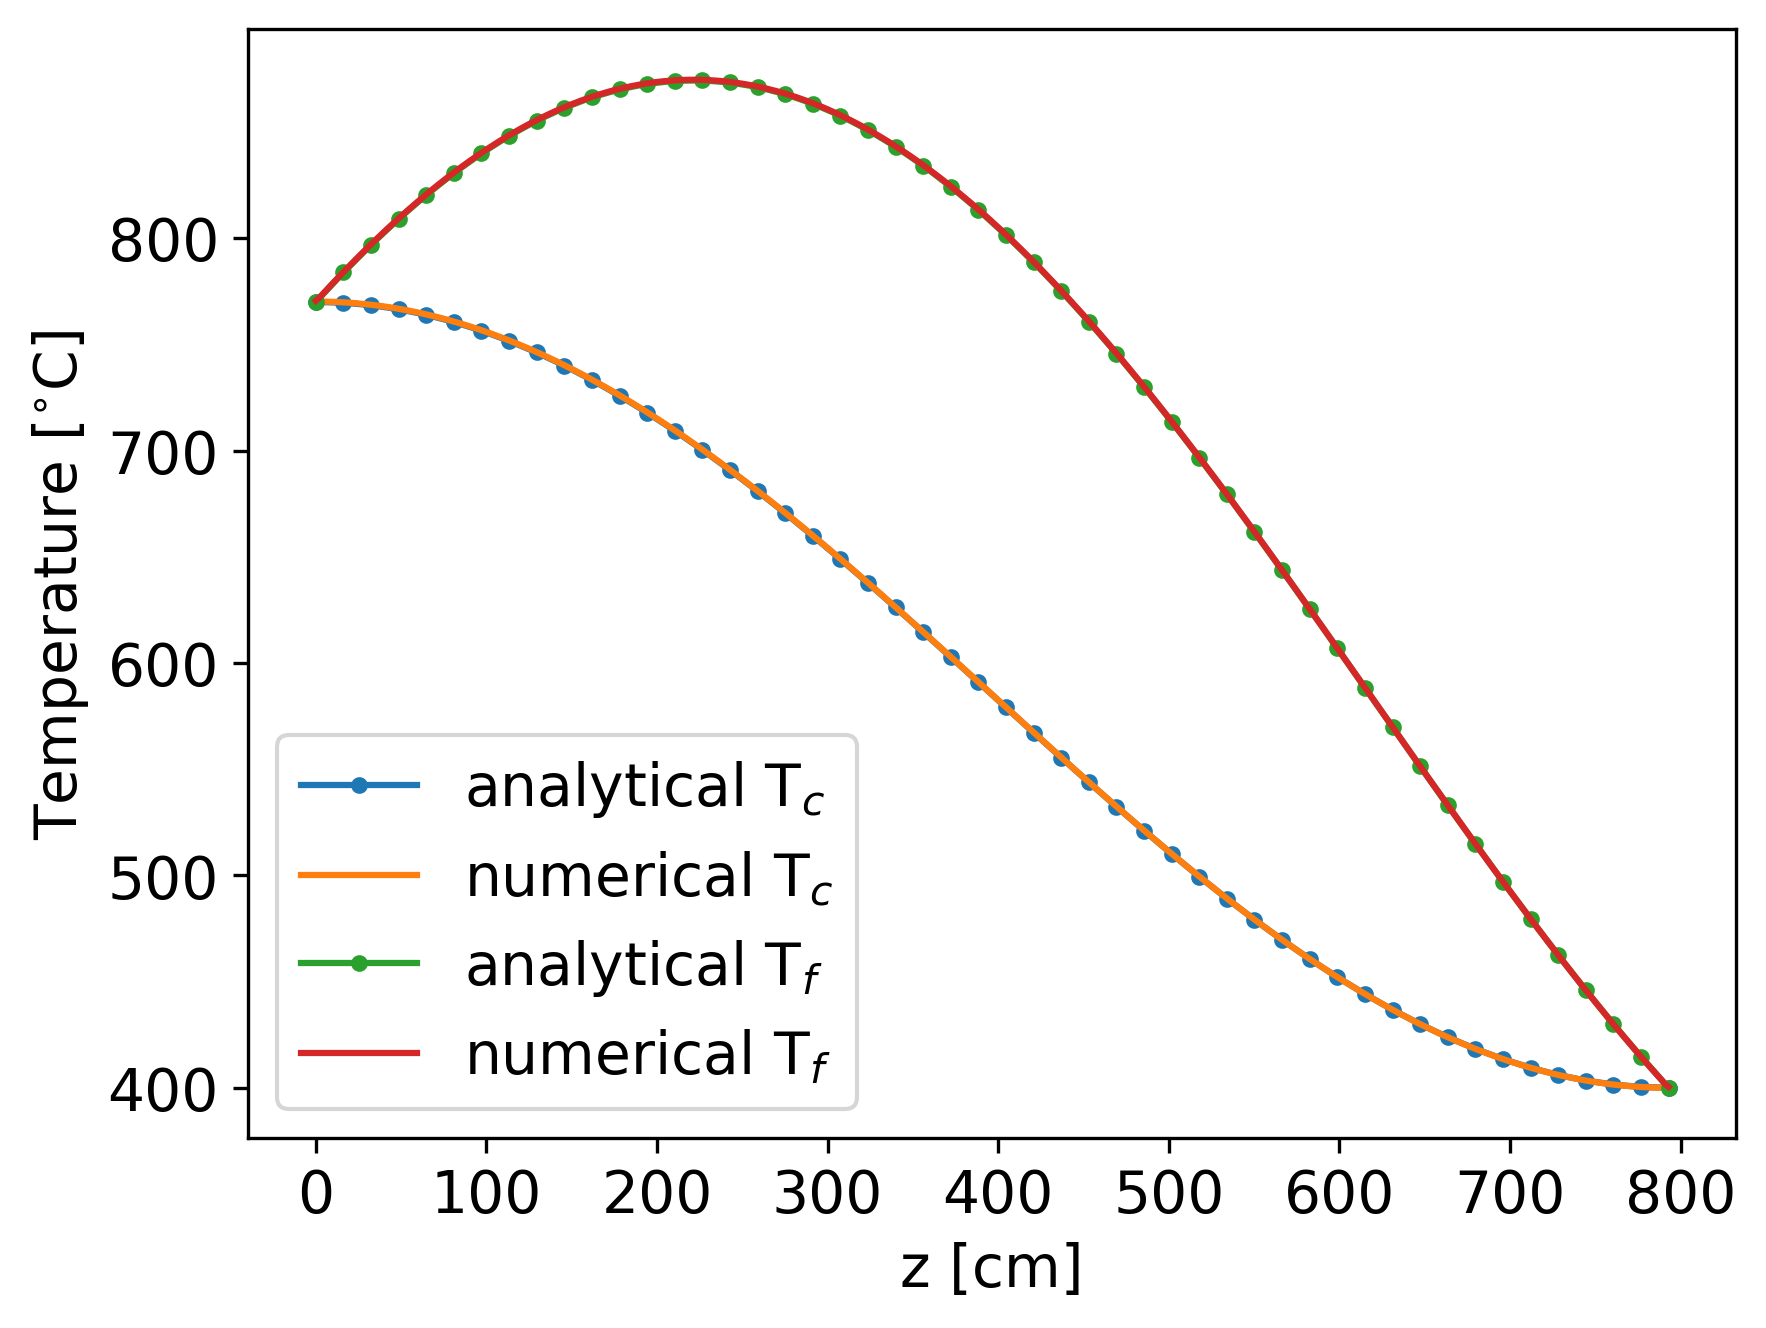
\includegraphics[width=0.45\textwidth]{figures-thermal/2D-preliminar-axial}
    }
    \subfloat[Radial temperature at z=396.5 cm.]{
        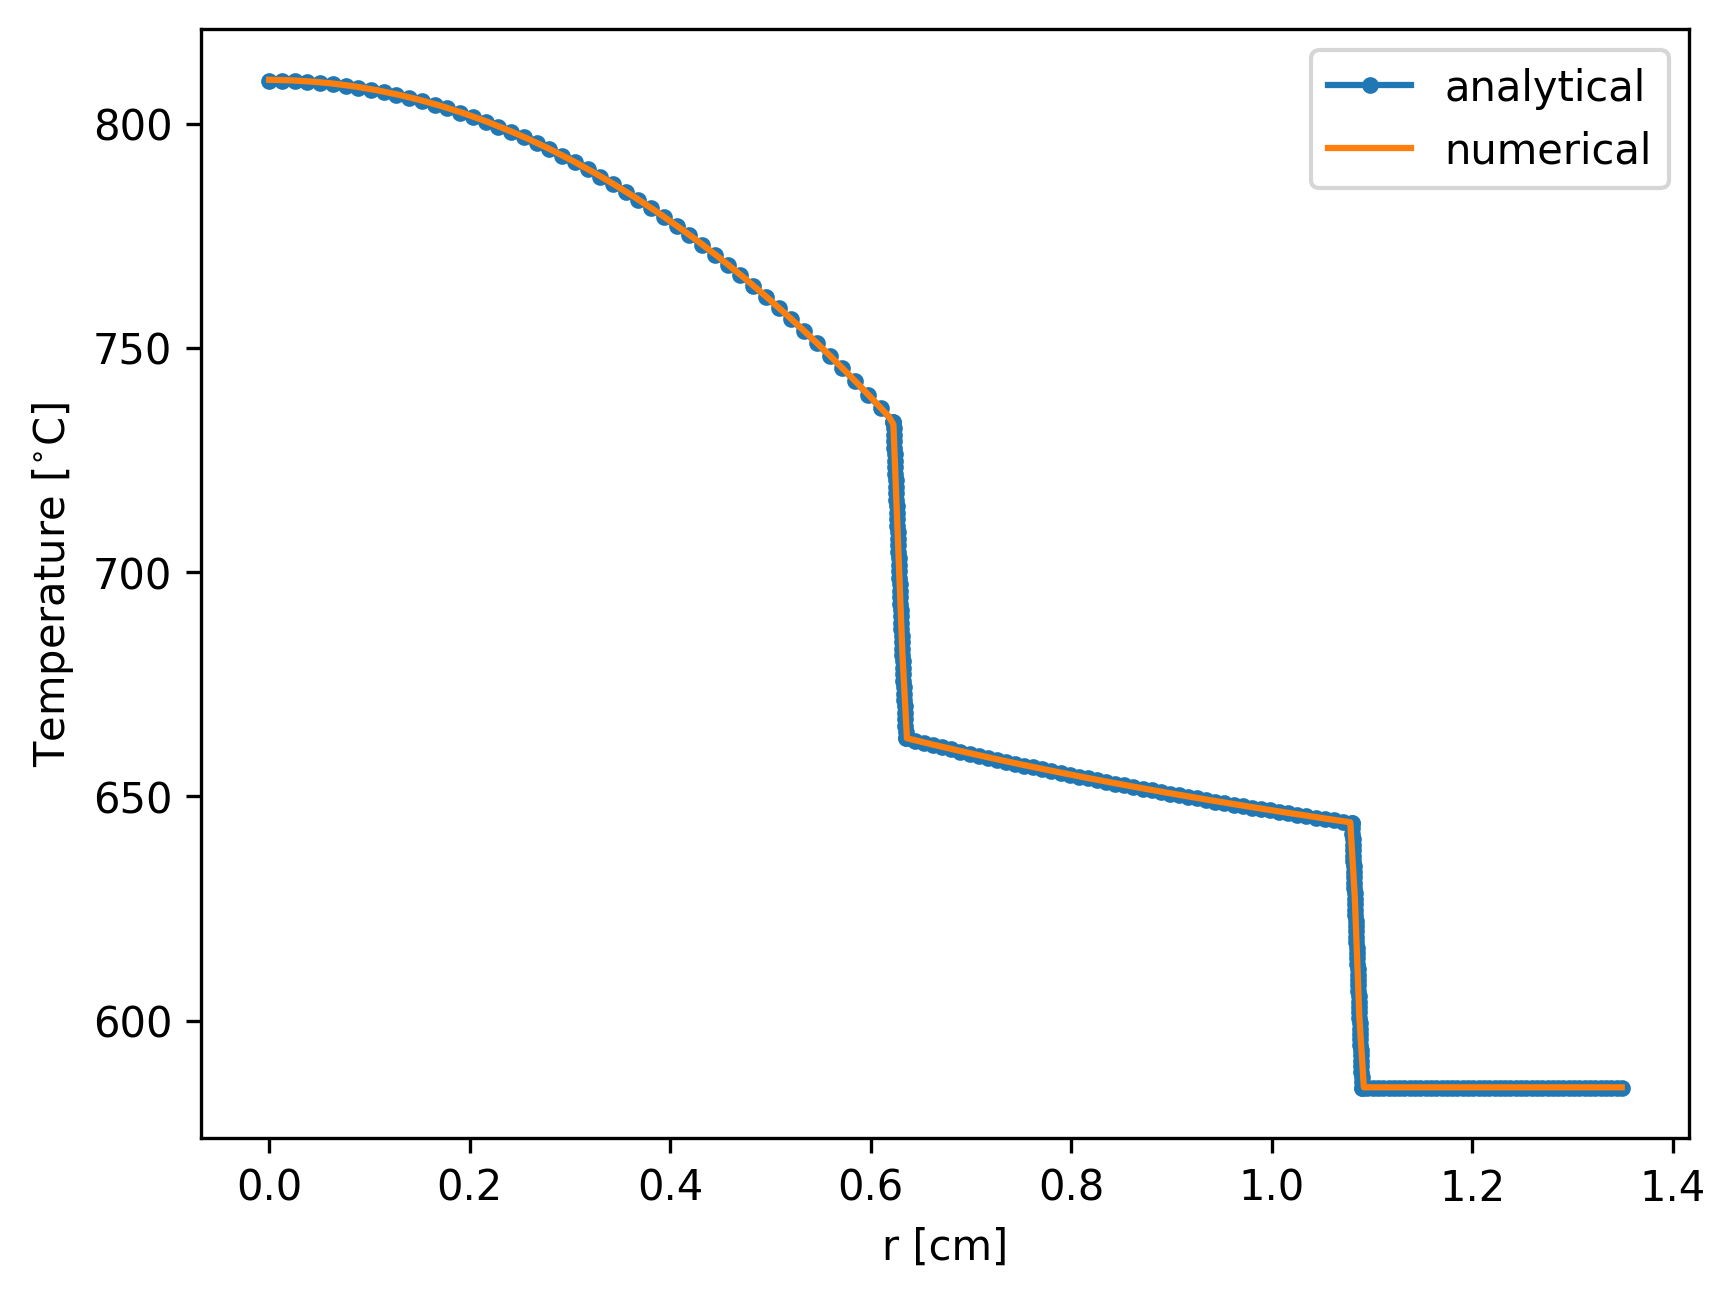
\includegraphics[width=0.45\textwidth]{figures-thermal/2D-preliminar-radial}
    }
	\hfill
    \caption{Temperature profiles.}
	\label{fig:th-ver-results}
\end{figure}

\section{Unit cell problem}

This section will solve the unit cell problem in the hot spot of an HTGR.

\section{Fuel assembly}

This section will calculate the heat profile of a fuel assembly of a HTGR.

\section{Full core}

This section will extend the methodology to a fullcore problem and it will inted to solve Exercise 2 of Phase I of the OECD/NEA MHTGR-350 Benchmark.




\section{Neutronics and Thermal-fluids Coupling}

3 options:
- Heterogeneous model
- Homogenized media and sub-channel unit cell model
- Porous media model


